\documentclass[conference]{IEEEtran}
\IEEEoverridecommandlockouts
\usepackage[utf8]{inputenc}
\usepackage{cite}
\usepackage{amsmath,amssymb,amsfonts}
\usepackage{algorithmic}
\usepackage{algorithm} 
\usepackage{graphicx}
\usepackage{textcomp}
\usepackage{xcolor}
\usepackage{booktabs}
\usepackage{array}
\usepackage{multirow}
\usepackage{url}
\usepackage{float}
\usepackage{caption}
\usepackage{subcaption}
\usepackage{enumitem}
\usepackage{makecell}
\usepackage{adjustbox}
\usepackage{tikz}
\usepackage{hyperref}
\usepackage{placeins}

\usetikzlibrary{shapes.geometric, arrows.meta, positioning, fit, backgrounds, calc, shadows, shapes}
\linespread{1.5}\selectfont 
\setlength{\parskip}{1.5em plus 0.2em minus 0.2em}
\setlength{\parindent}{0pt}
\definecolor{myblue}{RGB}{0, 114, 189}
\definecolor{myred}{RGB}{217, 83, 25}
\definecolor{mygreen}{RGB}{119, 172, 48}
\definecolor{myorange}{RGB}{237, 177, 32}
\definecolor{mygray}{RGB}{128, 128, 128}
\makeatletter
\newcommand{\REQUIRE}{\item[\textbf{Require:}]}
\newcommand{\ENSURE}{\item[\textbf{Ensure:}]}
\makeatother
\renewcommand{\arraystretch}{1.5} 
\renewcommand\theadfont{\bfseries\footnotesize}
\renewcommand{\arraystretch}{1.5}
\def\BibTeX{{\rm B\kern-.05em{\sc i\kern-.025em b}\kern-.08em
    T\kern-.1667em\lower.7ex\hbox{E}\kern-.125emX}}



\begin{document}

\title{MediXAI: Multimodal AI for Prescription Analysis and Personalized Health Monitoring --- A Comprehensive Review}

\author{\IEEEauthorblockN{1\textsuperscript{st} Md. Momin Ali Rifat}
\IEEEauthorblockA{\textit{Dept. of CSE} \\
\textit{University of Asia Pacific}\\
Dhaka, Bangladesh\\
23201009@uap-bd.edu}
\and
\IEEEauthorblockN{2\textsuperscript{nd} Md. Nazmuz Saif}
\IEEEauthorblockA{\textit{Dept. of CSE} \\
\textit{University of Asia Pacific}\\
Dhaka, Bangladesh \\
23201023@uap-bd.edu}
\and
\IEEEauthorblockN{3\textsuperscript{rd} Tahsin Rahman Khan}
\IEEEauthorblockA{\textit{Dept. of CSE} \\
\textit{University of Asia Pacific}\\
Dhaka, Bangladesh \\
23201050@uap-bd.edu}
}

\maketitle




\begin{abstract}
The global healthcare system continues to face critical challenges in medical prescription interpretation, drug interaction detection, and continuous personalized health monitoring, which significantly affect patient safety and treatment effectiveness. Medication errors caused by illegible handwritten prescriptions, incorrect dosage interpretation, and undetected adverse drug interactions remain a major cause of preventable patient harm worldwide, highlighting the urgent need for intelligent automated solutions. This review paper presents a comprehensive analysis of \textit{MediXAI}, a conceptual multimodal artificial intelligence framework that integrates prescription analysis and personalized health monitoring into a unified intelligent healthcare pipeline designed to improve accuracy and reliability in clinical decision support systems. The review mainly focuses on the application of multimodal AI techniques in handwritten prescription recognition, medication analysis, disease prediction, remote patient monitoring, and explainable healthcare systems for improving transparency and trust in AI-driven medical applications. The paper reviews recent studies published between 2020 and 2026 related to Optical Character Recognition (OCR), Natural Language Processing (NLP), computer vision, multimodal large language models, wearable healthcare technologies, and Explainable Artificial Intelligence (XAI), covering both foundational and state-of-the-art approaches in the field. The reviewed studies demonstrate significant improvements in prescription recognition accuracy, automated medication analysis, and patient monitoring performance using deep learning and multimodal AI approaches across different experimental settings. However, the analysis also identifies several research challenges, including limited clinical validation, multilingual limitations, data privacy concerns, and the lack of fully integrated cross-modal healthcare frameworks suitable for real-world deployment. Overall, this review provides a structured overview of current advancements, research gaps, and future directions for developing intelligent, scalable, and trustworthy AI-driven healthcare systems.
\end{abstract}


\begin{IEEEkeywords}
Multimodal AI, Prescription Analysis, Optical Character Recognition, Personalized Health Monitoring, Deep Learning, Explainable AI, Natural Language Processing
\end{IEEEkeywords}













\section{Introduction}
\label{sec:introduction}
Healthcare systems across the globe are currently undergoing a fundamental transformation driven by rapid and unprecedented advances in artificial intelligence, machine learning, and deep learning. Despite these technological strides, several critical and persistent challenges continue to plague everyday clinical practice, particularly in resource-constrained environments. Handwritten medical prescriptions remain the dominant communication medium between physicians and pharmacists in many developing countries, including India, Bangladesh, and numerous regions across Africa and Southeast Asia \cite{chandra2019prescription,vimbi2024brain}. The reliance on manual, handwritten documentation introduces a significant bottleneck in the efficiency of healthcare delivery. The World Health Organization has reported that medication errors affect approximately one in every ten patients globally, with a significant proportion linked to illegible prescriptions and miscommunication of drug names, dosages, and instructions \cite{sharjeel2025ai}. This statistic underscores a critical public health issue that requires immediate technological intervention.

The severity of this problem has been widely discussed and documented in previous studies. Researchers have consistently highlighted that adverse drug reactions caused by undetected drug-drug interactions are among the leading causes of preventable morbidity in hospitalized patients \cite{babu2024aidriven}. In addition, Bari et al. stated that handwriting variability among physicians contributes to nearly 60\% of medication-related errors in clinical environments \cite{devi2026endtoend}. These findings clearly indicate the urgent need for intelligent systems capable of accurately interpreting prescriptions and supporting safe medication management. Without robust automated solutions, the risk to patient safety remains unacceptably high, particularly in settings where medical professionals are overburdened.

The importance of this topic lies in improving patient safety, reducing medical errors, and enhancing healthcare efficiency. Intelligent systems that combine prescription analysis with patient monitoring can significantly reduce the workload of healthcare professionals while ensuring more accurate and personalized treatment decisions. Therefore, developing reliable AI-driven healthcare frameworks has become a critical research direction for the next decade. By automating routine cognitive tasks, healthcare providers can focus more on patient care and complex clinical reasoning.

Previous studies suggested that traditional healthcare AI systems generally operate in isolated pipelines. The work in \cite{gudi2025enhancing} demonstrated that prescription images can be converted into text, while NLP-based methods extract medical entities such as drug names and dosages from text data. However, these systems often function independently without integration across modalities. This limitation reduces their effectiveness in real-world clinical decision-making scenarios, where multiple data sources must be considered simultaneously to form a holistic view of the patient's condition. A holistic approach is necessary to move beyond simple digitization towards actionable clinical intelligence.

Recent research demonstrated that Multimodal Large Language Models such as LLaVA, Idefics2, and Qwen-VL can effectively process both visual and textual medical data \cite{mankash2024mirage,intuitionlabs2026pharma}. The MIRAGE framework demonstrated 82\% accuracy in extracting medication information from handwritten prescriptions \cite{gifu2022aibacked,mankash2024mirag}. Concurrently, wearable sensor technologies have enabled continuous monitoring of physiological signals such as heart rate and oxygen saturation \cite{kin2024medical}. These developments indicate strong potential for integrating multimodal data in healthcare applications. The convergence of vision, language, and sensor data represents the frontier of medical AI.

Furthermore, explainable AI has been widely studied to improve transparency in medical systems. The researchers discussed that LIME and SHAP improve interpretability in disease detection models and increase clinical trust \cite{nguyen2021evaluation}. Similarly, evaluation studies demonstrated that CAM-based visualization techniques effectively explain deep learning decisions in medical imaging tasks \cite{kumar2025doctors,singaravelu2018prescription}. Trust is a prerequisite for the adoption of AI in sensitive domains like healthcare, making explainability a non-negotiable feature of modern systems.
nguyen2021evaluation
In this context, this review introduces MediXAI, a multimodal AI framework for prescription analysis and personalized health monitoring with explainable AI. The framework consists of four main components: (i) a Prescription OCR module for handwritten and printed prescription recognition; (ii) an NLP and drug safety module for extracting medication information and detecting drug interactions; (iii) a health monitoring module for wearable sensor data fusion; and (iv) an explainable AI module using LIME, SHAP, and Grad-CAM for transparent decision-making.

The main objective of this review paper is to analyze current research in OCR, NLP, computer vision, multimodal deep learning, wearable healthcare systems, and explainable AI. The work in this paper compares different methodologies, datasets, performance results, and limitations across eighteen selected studies and identifies major research gaps for future improvement.

The remainder of this paper is organized as follows. Section~\ref{sec:Novelty} describes the novelty and contribution of this review. Section~\ref{sec:methodology} presents the review methodology and algorithmic workflows. Section~\ref{sec:background} provides background concepts. Section~\ref{sec:literature} presents the literature review. Section~\ref{sec:comparative} shows comparative analysis. Section~\ref{sec:pipeline} introduces the MediXAI framework. Section~\ref{sec:challenges} discusses challenges and research gaps. Section~\ref{sec:future} presents future directions. Section~\ref{sec:conclusion} concludes the paper.







\section{Novelty and Contribution}
\label{sec:Novelty}

The primary novelty of this review lies in the systematic integration of three traditionally isolated research domains-prescription OCR, personalized health monitoring, and explainable AI-into one unified multimodal healthcare framework termed MediXAI. While numerous surveys address these topics individually, no existing review connects them under a single conceptual pipeline. This integration is clinically significant because a prescription becomes truly meaningful only when the healthcare system can also monitor whether the prescribed treatment is effective and whether the patient is responding safely.

\textbf{Contribution 1: Systematic Review and Analysis:}
This review presents a comprehensive analysis of eighteen research papers published between 2021 and 2026. Unlike previous surveys that might focus on a single modality (e.g., text-only OCR), this work provides a holistic comparison across general deep learning approaches, advanced multimodal vision-language models, and explainability techniques, thereby offering a complete picture of the current landscape.

\textbf{Contribution 2: Novel Categorization and Classification:}
A key methodological contribution of this review is the novel three-category classification of the reviewed literature. This classification clarifies the evolutionary trajectory from traditional single-modality approaches (Category A) to state of the art multimodal systems (Category B) and emerging explainable AI methodologies (Category C). This categorization aids researchers in quickly identifying suitable methodologies for specific clinical needs.

\textbf{Contribution 3: Comprehensive Attribute Comparison:}
This review provides a granular, ten attribute comparison of every reviewed paper (covering title, year, dataset, method, result, error analysis, limitations, future work, strong points, weak points, and dataset links). This depth of comparison allows for a fine-grained analysis that is often missing in broader medical AI surveys.

\textbf{Contribution 4: The MediXAI Conceptual Pipeline:}
The review proposes the MediXAI conceptual framework a five stage architecture (Input Acquisition, Preprocessing, AI Processing, Multimodal Fusion, Clinical Feedback). This proposed architecture serves as a theoretical blueprint for integrating disjointed systems into a cohesive unit, specifically addressing the gap between static prescription analysis and dynamic patient monitoring.

\textbf{Contribution 5: Identification of Critical Gaps:}
Building on the comparative analysis, this review identifies critical research gaps that hinder the transition from experimental research to real world clinical application. Specifically, it highlights the absence of cross modal fusion (connecting prescription digitization with wearable monitoring), the lack of multilingual support for non-English prescriptions, insufficient clinical validation of proposed models, and the need for privacy-preserving approaches like Federated Learning in healthcare.

\textbf{Justification for Novelty:}
Existing literature often treats these domains in isolation. For instance, many reviews focus solely on OCR accuracy metrics \cite{mankash2024mirage,kumar2025doctors} or general predictive analytics \cite{intuitionlabs2026pharma,talekar2025interpreting} without considering how these systems interact with the patient's real-time physiological state. Others focus purely on the theoretical aspects of Explainable AI \cite{berha2018evaluation}. By reviewing the eighteen specific papers and their methodologies, this review demonstrates that the "siloed" approach is no longer sufficient. The MediXAI framework is presented as the necessary next step: a multimodal, explainable system that closes the loop between the prescription (the plan) and the patient (the reality).

\textbf{Examples of Specific Contributions:}
\textit{New Comparison Method:} The review compares the effectiveness of traditional CNN/LSTM architectures against modern Vision-Language Models (e.g., MIRAGE using LLaVA \cite{priya2026medicalocr}) within the same document.
\textit{Updated Survey of Recent Works:} Unlike older surveys that may cite literature up to 2020-2022, this review includes the latest 2026 studies (e.g., End-to-End Pipeline \cite{srinivasa2020analysis}).
\textit{Research Gap Identification:} It explicitly points out that while accuracy is improving (reaching 99.6\% in some studies \cite{datta2025preserving}), the lack of privacy integration and real world clinical validation remains a major unsolved problem.

\begin{enumerate}[label=(\roman*)]
    \item A systematic review and comparative analysis of eighteen research papers (2021-2026) across three thematic categories: general prescription OCR, advanced multimodal prescription OCR, and explainable AI in healthcare.
    
    \item A novel three-category classification of the reviewed literature that clarifies the relationship between traditional OCR approaches, modern vision-language model approaches, and XAI frameworks.
    
    \item A detailed ten-attribute comparison of every reviewed paper covering title, year, dataset, method, results, error analysis, limitations, future work, strong points, and weak points with dataset links.
    
    \item The proposal of the MediXAI conceptual pipeline with a five-stage architecture: input acquisition, prescription digitization, multimodal fusion, monitoring and recommendation, and explainable clinical feedback.
    
    \item Identification of critical research gaps including the absence of cross-modal fusion connecting prescription analysis with patient monitoring, limited multilingual support, insufficient clinical validation, and the need for privacy-preserving federated learning approaches.
\end{enumerate}









\section{Methodology}
\label{sec:methodology}

The methodology is organized into two main steps: (1) explaining the fundamental concepts, models, and algorithms required to understand the domain, and (2) conducting a structured systematic literature review including paper selection, categorization, and data extraction.


To ensure a clear understanding of the reviewed studies, this step defines the core concepts, models, and system components used in handwritten prescription analysis and multimodal healthcare AI systems.

\subsubsection{Definitions of Core Concepts}\\

\textbf{Optical Character Recognition (OCR):}
OCR is a computer vision technique that converts handwritten or printed text into machine-readable format. It is the first stage of prescription digitization systems.

\textbf{Natural Language Processing (NLP):}
NLP enables machines to understand and interpret human language. In healthcare, it is used for extracting medical entities such as drug names, dosage, and instructions.

\textbf{Multimodal AI:}
Multimodal AI combines multiple data sources such as images and text to improve prediction and understanding. It integrates vision and language models for prescription analysis.

\textbf{Explainable AI (XAI):}
XAI provides interpretability to AI models using methods such as LIME, SHAP, and Grad-CAM, which are essential for trustworthy medical decision systems.

\subsubsection{Core Models and Architectures}

The reviewed literature is based on deep learning architectures. CNNs are used for feature extraction from images, while RNNs (LSTM/GRU) are used for sequence modeling. Transformer-based models such as Vision Transformer (ViT), Swin Transformer, and vision-language models (e.g., LLaVA, Donut) are widely used for end-to-end prescription understanding.

\subsubsection{System Architecture Overview}

The overall workflow of the proposed prescription analysis system is shown in Figure~\ref{fig:pipeline}.


\begin{figure}[H]
\centering

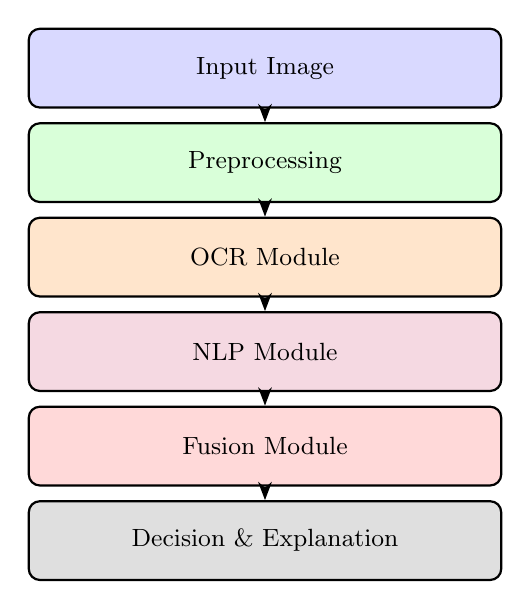
\begin{tikzpicture}[
    node distance=1.2cm,
    every node/.style={font=\small},
    block/.style={
        rectangle,
        draw,
        rounded corners,
        text centered,
        minimum width=6cm,
        minimum height=1cm,
        thick
    },
    arrow/.style={thick,->,>=Stealth}
]

\node (input) [block, fill=blue!15] {Input Image};
\node (prep) [block, below of=input, fill=green!15] {Preprocessing};
\node (ocr) [block, below of=prep, fill=orange!20] {OCR Module};
\node (nlp) [block, below of=ocr, fill=purple!15] {NLP Module};
\node (fusion) [block, below of=nlp, fill=red!15] {Fusion Module};
\node (output) [block, below of=fusion, fill=gray!25] {Decision \& Explanation};


\draw [arrow] (input) -- (prep);
\draw [arrow] (prep) -- (ocr);
\draw [arrow] (ocr) -- (nlp);
\draw [arrow] (nlp) -- (fusion);
\draw [arrow] (fusion) -- (output);

\end{tikzpicture}

\caption{End-to-end vertical pipeline of the proposed prescription analysis system}
\label{fig:pipeline}
\end{figure}

\subsubsection{Algorithmic Workflows for Personalized Treatment Recommendation (PTR)}

The following algorithms outline the core logic for Personalized Treatment Recommendation paradigms reviewed in this survey, ranging from content-based to hybrid filtering approaches.

\vspace{0.5em}

\begin{algorithm}[H]
\caption{Content-based filtering model for treatment recommendation}
\label{alg:content_based}
\begin{algorithmic}[1]
\REQUIRE Patient profile $P$, Treatment database $T$, Similarity function $Sim()$ \ENSURE Recommended treatments
\STATE Extract patient features from $P$
\STATE Extract treatment features from $T$
\STATE Initialize an empty list $R$
\FOR{each treatment $t_i$ in $T$}
    \STATE Compute similarity score $s_i = Sim(P, t_i)$
    \STATE Append $(t_i, s_i)$ to $R$
\ENDFOR
\STATE Sort $R$ based on similarity scores in descending order
\STATE Return Top-N treatments from $R$
\end{algorithmic}
\end{algorithm}

\vspace{1em}

\begin{algorithm}[H]
\caption{Collaborative-filtering based treatment recommendation}
\label{alg:collaborative}
\begin{algorithmic}[1]
\REQUIRE Matrix $M$, Patient $P_t$, Similarity $Sim()$ \ENSURE Recommended Treatments for $P_t$
\STATE Extract history $H_t$ of $P_t$ from $M$
\STATE Initialize list $S$
\FOR{each $P_i$ in $M$}
    \STATE $s_i \gets Sim(P_t, P_i)$
    \STATE Append $(P_i, s_i)$ to $S$
\ENDFOR
\STATE Sort $S$ by $s_i$ in descending order
\STATE Select top-$k$ similar patients
\STATE Initialize list $T$
\FOR{each treatment $T_j$}
    \STATE Compute score $\hat{s}_j$ via weighted CF
    \STATE Append $(T_j, \hat{s}_j)$ to $T$
\ENDFOR
\STATE Sort $T$ by $\hat{s}_j$ in descending order
\STATE Return Top-N treatments from $T$
\end{algorithmic}
\end{algorithm}

\vspace{1em}

\begin{algorithm}[H]
\caption{Knowledge-based filtering treatment recommendation}
\label{alg:knowledge}
\begin{algorithmic}[1]
\REQUIRE Patient Profile $P$, Knowledge Base $K$, Rule-Based Engine $R$ \ENSURE Recommended Treatments $T$
\STATE Extract patient-specific data $D$ (e.g., medical history, symptoms, risk factors) from $P$
\STATE Retrieve clinical guidelines and expert knowledge from $K$
\STATE Initialize empty list $S$
\FOR{each candidate treatment $t$}
    \STATE Evaluate $t$ using rule-based matching via $R$
    \STATE Compute relevance score $r_t$ based on:
    \STATE \quad Alignment with clinical guidelines
    \STATE \quad Treatment efficacy from prior outcomes
    \STATE \quad Patient-specific risk and contraindication profiles
    \STATE Append $(t, r_t)$ to $S$
\ENDFOR
\STATE Sort $S$ by $r_t$ in descending order
\STATE Select top-$N$ treatments
\STATE Return Recommended treatments $T$
\end{algorithmic}
\end{algorithm}

\vspace{1em}

\begin{algorithm}[H]
\caption{Hybrid filtering treatment recommendation}
\label{alg:hybrid}
\begin{algorithmic}[1]
\REQUIRE Patient profile $P$, Treatment database $D$, Similarity function $Sim()$, Knowledge base $KB$, Fusion Method $Fusion\_Method$ \ENSURE Recommended Treatments $T$
\STATE Extract patient-specific features from $P$
\STATE Retrieve available treatments from $D$
\STATE \textbf{Step 1: Content-Based Filtering}
\FOR{each treatment $t$ in $D$}
    \STATE Compute similarity score $s_{CB}(t) = Sim(P, t)$
\ENDFOR
\STATE \textbf{Step 2: Collaborative Filtering}
\STATE Identify top-$k$ similar patients
\STATE Predict treatment scores $s_{CF}(t)$ using collaborative filtering
\STATE \textbf{Step 3: Knowledge-Based Filtering}
\FOR{each treatment $t$ in $D$}
    \STATE Evaluate $t$ using knowledge base $KB$ and assign score $s_{KB}(t)$
\ENDFOR
\STATE \textbf{Step 4: Hybrid Fusion}
\FOR{each treatment $t$ in $D$}
    \STATE Compute final score $s_{final}(t) = Fusion\_Method(s_{CB}(t), s_{CF}(t), s_{KB}(t))$
\ENDFOR
\STATE \textbf{Step 5: Ranking and Selection}
\STATE Rank all treatments in $D$ by $s_{final}(t)$ in descending order
\STATE Return Top-N treatments
\end{algorithmic}
\end{algorithm}


\subsection{Step 2: Systematic Literature Review Process}

\subsubsection{Research Questions}

\begin{itemize}
    \item \textbf{RQ1}: What are the current state-of-the-art methods for prescription recognition?
    \item \textbf{RQ2}: How do multimodal AI systems compare with traditional OCR pipelines?
    \item \textbf{RQ3}: What role does Explainable AI play in healthcare decision systems?
    \item \textbf{RQ4}: What are the major limitations of existing systems?
    \item \textbf{RQ5}: What research gaps remain in multimodal frameworks?
\end{itemize}


\subsubsection{Paper Selection and Categorization}

Were shortlisted and 18 were selected for final review.

\begin{itemize}
    \item \textbf{Category A}: OCR-based methods
    \item \textbf{Category B}: Multimodal AI systems
    \item \textbf{Category C}: Explainable AI methods
\end{itemize}

\subsubsection{Data Extraction Framework}

For each paper, the following attributes were extracted: author, year, dataset, methodology, contribution, advantages, limitations, and results.

Table~\ref{tab:summary_method} presents the comparative summary of all selected studies.

\begin{table*}[!htbp]
\centering
\caption{Summary of Reviewed Papers Used in this Review}
\label{tab:summary_method}
\footnotesize
\begin{tabular}{|c|l|c|l|c|l|}
\hline
\textbf{ID} & \textbf{Paper (Short Title)} & \textbf{Year} & \textbf{Primary Method} & \textbf{Best Result} & \textbf{Category} \\
\hline
A1 & End-to-End Prescription Pipeline & 2026 & OCR + NLP Pipeline & Char: 71\%, Word: 84\% & OCR-based \\
A2 & AI-Driven Predictive Analytics & 2024 & LR, RF, SVM, CNN, RNN & Improved prediction & OCR-based \\
A3 & AI-backed OCR in Healthcare & 2022 & CNN + CRNN & 73--82\% & OCR-based \\
A4 & AI-Based OCR for Prescriptions & 2025 & CNN-LSTM + Tesseract + NLP & 92\% accuracy & OCR-based \\
A5 & Doctors' Handwriting Recognition & 2025 & CNN+RNN+LSTM+CTC & $\sim$90\%+ & OCR-based \\
A6 & MedicalOCR: Prescription Recog. & 2026 & OCR + CNN & Improved digitization & OCR-based \\
A7 & Enhancing OCR with ANN & 2025 & Hybrid OCR + ANN/MLP & CRR: 94.5\% & OCR-based \\
\hline
B1 & MIRAGE (Indian Prescriptions) & 2024 & LLaVA, Idefics2, QWEN VL & 82\% F1 & Multimodal AI \\
B2 & Interpreting Doctors' Notes & 2025 & CNN-LSTM + Tesseract & 91.3\% char & Multimodal AI \\
B3 & AI Solution Illegible Handwriting & 2025 & OCR + NLP + Dual RAG & 92\% overall & Multimodal AI \\
B4 & Preserving Medical Information & 2025 & YOLO + OCR + Spell Corr. & 99.6\% ROI & Multimodal AI \\
B5 & Prescription OCR (Donut) & 2024 & Donut (Swin + BART) & Qualitative & Multimodal AI \\
B6 & Pharma Document AI Benchmark & 2025 & VLMs + BioBERT & 94--96\% & Multimodal AI \\
B7 & Prescription Reader OCR & 2025 & Multi-agent AI + YOLO & Printed: 97--99\% & Multimodal AI \\
\hline
C1 & LIME \& SHAP in Alzheimer's & 2024 & ML/DL + LIME + SHAP & Up to 99.9\% & Explainable AI \\
C2 & SHAP \& Grad-CAM in HAR & 2025 & ML/DL + SHAP + Grad-CAM & Improved interp. & Explainable AI \\
C3 & XAI Practical Guide & 2023 & ML + LIME + SHAP & Demo results & Explainable AI \\
C4 & Evaluation of SHAP, LIME, CAM & 2021 & DL + SHAP + LIME + CAM & CAM best visual. & Explainable AI \\
\hline
\end{tabular}
\end{table*}








\section{Background and Basic Concepts}
\label{sec:background}

\subsection{Optical Character Recognition in Healthcare}

Optical Character Recognition is the computational process of converting images of handwritten or printed text into machine-readable characters. In the healthcare domain, OCR faces unique challenges due to the extreme variability of physician handwriting, non-standard abbreviations, and poor image quality from faxed or scanned documents \cite{mankash2024mirage,intuitionlabs2026pharma,babu2024aidriven}.

Traditional OCR systems such as Tesseract employ a pipeline of image binarization, text line segmentation, character segmentation, and recognition using Hidden Markov Models or multi-layer perceptrons. While effective for printed text, these systems achieve only moderate accuracy (70--80\%) on handwritten medical prescriptions \cite{talekar2025interpreting}. Modern deep learning approaches have significantly improved performance by replacing handcrafted feature extraction with learned representations. CNN architectures extract spatial features, while recurrent networks such as LSTM and Bi-LSTM capture sequential dependencies in text. The Connectionist Temporal Classification (CTC) loss function has become standard for sequence-to-sequence recognition without requiring explicit character segmentation \cite{mankash2024mirage,intuitionlabs2026pharma}.

More recently, transformer-based architectures have emerged as the state-of-the-art. The Donut model combines a Swin Transformer encoder with a BART decoder to provide OCR-free end-to-end document understanding \cite{mankash2024mirage}. Vision-Language Models such as PaliGemma, LLaVA, Qwen-VL, and InternVL have achieved 94--96\% accuracy on pharmaceutical documents by jointly processing visual and textual features \cite{sharjeel2025ai}.

\subsection{Natural Language Processing for Drug Safety}

Natural Language Processing enables the extraction of structured information from unstructured clinical text. Named Entity Recognition systems trained on biomedical corpora can identify medication names, dosages, frequencies, and routes of administration. Drug-drug interaction detection represents a critical safety application where transformer-based models such as BioBERT have demonstrated strong performance in identifying interaction-containing sentences from clinical text \cite{singaravelu2018prescription}. The integration of NLP with OCR output creates a complete prescription understanding pipeline, although error propagation from OCR to NLP remains a significant challenge \cite{berha2018evaluation}.

\subsection{Personalized Health Monitoring}

Personalized health monitoring refers to the continuous or periodic observation of patient-specific health data to track disease progression, treatment response, and adverse effects. Modern wearable devices can measure heart rate variability, electrocardiogram, photoplethysmography, blood oxygen saturation, skin temperature, and electrodermal activity \cite{talekar2025interpreting}. AI-driven analysis of multimodal wearable sensor data enables predictive health analytics, anomaly detection, and adaptive treatment monitoring.

\subsection{Explainable AI in Clinical Decision Support}

Explainable AI encompasses methods that make the predictions of machine learning and deep learning models understandable to human users. In healthcare, explainability is essential for clinical trust, regulatory compliance, and error detection \cite{nguyen2021evaluation}. The three most widely used XAI frameworks are:

\begin{itemize}
    \item \textbf{LIME} (Local Interpretable Model-agnostic Explanations): Generates local surrogate models to explain individual predictions \cite{gifu2022aibacked,talekar2025interpreting}.
    \item \textbf{SHAP} (SHapley Additive exPlanations): Uses game-theoretic Shapley values to compute feature contributions \cite{gifu2022aibacked,berha2018evaluation}.
    \item \textbf{Grad-CAM} (Gradient-weighted Class Activation Mapping): Produces visual heatmaps showing which image regions influenced CNN predictions \cite{berha2018evaluation,devi2026endtoend}.
\end{itemize}

\subsection{Multimodal Fusion Strategies}

Multimodal fusion combines information from different data modalities into a unified representation. Three primary strategies exist: \textit{early fusion}, which concatenates raw features before processing; \textit{late fusion}, which combines predictions from modality-specific models at the decision level; and \textit{intermediate fusion}, which merges learned representations at hidden layers. The optimal strategy depends on data quality, clinical task, and computational constraints \cite{intuitionlabs2026pharma,mankash2024mirage}.

\section{Literature Review}
\label{sec:literature}

\subsection{Category A: Handwritten Prescription OCR --- General Approaches}

\subsubsection{A1: End-to-End Pipeline for Handwritten Prescription Understanding (2026)}

The researchers in \cite{devi2026endtoend} presented an end-to-end pipeline integrating OCR with clinical NLP for handwritten prescription understanding. The primary focus of this study was error propagation analysis, examining how OCR errors cascade into downstream NLP entity extraction tasks. Using public handwritten text datasets combined with clinical NLP benchmarks, the pipeline achieved character-level accuracy of 71\% and word-level accuracy of 84\%. Medication name extraction ranged between 85--90\%, while dosage extraction achieved 70--80\%. The key contribution lies in demonstrating that a 10\% character error rate in OCR can produce a 15--25\% degradation in NLP accuracy. The primary limitation is that no new algorithm was proposed; the study served as a system-level evaluation using existing components.

\subsubsection{A2: AI-Driven Healthcare: Predictive Analytics (2024)}

The work presented in \cite{gudi2025enhancing} provided a broad survey of machine learning and deep learning methods for predictive analytics in disease diagnosis and treatment. The study examined multiple techniques including Logistic Regression, Random Forest, SVM, Gradient Boosting, CNN, and RNN applied to Electronic Health Records, medical imaging data, genomic datasets, and wearable device data. The study demonstrated improved disease prediction accuracy across multiple clinical scenarios. However, the researchers acknowledged that model errors arise primarily from noisy medical data, missing EHR values, dataset bias, and misclassification in complex cases. Data privacy concerns, algorithmic bias, and integration difficulties with hospital information systems were identified as major limitations.

\subsubsection{A3: AI-backed OCR in Healthcare (2022)}

Pavithiran et al.\ \cite{gifu2022aibacked} conducted a comparative study of CNN and CRNN architectures for medical handwriting recognition. The study utilized two datasets: the Kaggle ASL dataset containing 372,451 images across 26 classes and a Romanian medical handwritten corpus comprising 7,700 samples from 17 doctors. The CNN model achieved 70--80\% accuracy, while the CRNN architecture combining CNN with Bi-LSTM and CTC loss slightly improved performance to 73--82\%. The researchers observed overfitting after approximately 18 training epochs and noted that class imbalance significantly affected recognition performance. The study introduced a valuable Romanian medical OCR corpus but was limited by the absence of diacritics support and a production-level deployment system.

\subsubsection{A4: AI-Based OCR System for Prescription Recognition (2025)}

The system proposed in \cite{gifu2022aibacked} combined CNN-LSTM with Tesseract OCR and NLP in a hybrid architecture for handwritten medical prescription recognition and interpretation. Using a real-world multilingual annotated dataset, the system achieved approximately 92\% accuracy, 90\% precision, and 88\% recall with a processing speed of 1.5 seconds per image. The researchers deployed the system as a web application using Streamlit, demonstrating practical healthcare utility. Errors occurred primarily with rare medical abbreviations, poor-quality images, and complex cursive handwriting. The main limitation was that the dataset was not publicly available, restricting reproducibility.

\subsubsection{A5: Doctors' Handwriting Recognition (2025)}

The study in \cite{intuitionlabs2026pharma} presented an end-to-end hybrid system combining CNN, RNN, LSTM, OCR, and CTC loss for physician handwriting recognition. Using curated and augmented public prescription datasets, the system achieved recognition performance exceeding 90\% with real-time processing under 5 seconds per image. The architecture incorporated fuzzy correction mechanisms to handle ambiguous characters. Persistent errors occurred in highly cursive writing, unclear strokes, and low-quality image noise. The researchers recommended future integration of Vision Transformers, BERT-based language models, and Explainable AI techniques including SHAP and Grad-CAM.

\subsubsection{A6: MedicalOCR: Doctor's Handwritten Prescription Recognition (2026)}

The MedicalOCR system \cite{chandra2019prescription} combined OCR with CNN and integrated NLP-based drug safety validation including interaction checking. The system successfully extracted medicine names, dosages, and instructions from handwritten prescriptions, reducing manual interpretation errors. The integration of drug interaction validation represented a significant advancement toward patient safety. However, performance depended heavily on image quality, and limited real-world clinical validation was conducted. The researchers proposed expanding the dataset and integrating transformer-based NLP for improved accuracy.

\subsubsection{A7: Enhancing OCR Accuracy using Artificial Neural Networks (2025)}

The study in \cite{srinivasa2020analysis} employed a hybrid OCR pipeline on a substantial dataset of 10,000 faxed prescription images with diverse handwriting styles. The system achieved Character Recognition Rate of 94.5\%, Word Recognition Rate of 90.3\%, and Page-level Accuracy Rate of 85.7\%, representing approximately 6--7\% improvement over baseline OCR. The experimental evaluation on a real-world dataset of meaningful size was a notable strength. However, the system remained partly constrained to ANN/MLP architectures and did not incorporate modern transformer-based OCR methods. Limited dataset diversity and English-only focus were identified as key limitations.

\subsection{Category B: Advanced Multimodal Prescription OCR}

\subsubsection{B1: MIRAGE --- Multimodal Recognition of Indian Prescriptions (2024)}

Mankash et al.\ \cite{mankash2024mirage} proposed MIRAGE, a multimodal framework for identifying and recognizing annotations in Indian general prescriptions. The study stands out for its exceptionally large dataset of 743,118 simulated handwritten prescriptions generated from 1,133 Indian doctors, with 100 records publicly released. The researchers fine-tuned three Multimodal Large Language Models---LLaVA 1.6, Idefics2, and QWEN VL---using LoRA and QLoRA quantization techniques with SigLIP and CLIP vision encoders backed by Mistral 7B as the language model. Idefics2 achieved the highest extraction accuracy of 82\%, followed by LLaVA at 79.8\%. The error analysis revealed that the CLIP vision encoder underperformed on handwritten text and that the LLM component could not compensate for vision encoder failures, creating a handwriting recognition bottleneck at the CLIP stage. Despite achieving higher accuracy than previous works, the 82\% performance level remains insufficient for unsupervised clinical deployment, and training required 13 days on six NVIDIA A6000 GPUs.

\subsubsection{B2: Interpreting Doctors' Notes (2025)}

The researchers in \cite{intuitionlabs2026pharma} developed a hybrid CNN-LSTM system combined with Tesseract OCR for interpreting handwritten physician notes. The system achieved 91.3\% character-level accuracy on real handwritten prescriptions preprocessed with OpenCV. The 8\% residual error rate was identified as potentially risky for medication safety. Errors occurred primarily in faded or smudged scans, noisy images, merged letters, and missing medical terminology. The study noted that Tesseract dependency and relatively slow processing speed of 1.8 seconds per image limited practical deployment. No semantic or medical validation layer was included.

\subsubsection{B3: AI Solution for Illegible Doctor Handwriting (2025)}

The RunPulse/AIQLabs study \cite{priya2026medicalocr} introduced a Custom OCR combined with NLP and Dual Retrieval Augmented Generation for processing illegible physician handwriting. Using a public dataset of 100+ real handwritten clinical notes augmented with 287 synthetic handwriting fonts, the system achieved 92\% overall accuracy, with performance varying by document type: 94--97\% for prescriptions and 90--94\% for clinical notes. The error analysis revealed that consumer-grade OCR systems lacking medical context led to 30\% more clarification calls. LLM hallucinations and dosage misreads remained significant concerns. The study emphasized that 92\% accuracy is insufficient for unsupervised clinical use and that human oversight remains necessary.

\subsubsection{B4: Preserving Medical Information from Prescriptions (2025)}

The study presented in \cite{babu2024aidriven} proposed a YOLO-based region of interest detection combined with OCR and spell correction for preserving medical information from multilingual prescriptions. The system achieved 99.6\% ROI detection accuracy and 96\% spell correction accuracy on annotations from real doctor prescriptions. The approach uniquely supported both handwritten and printed prescriptions with multilingual capability. However, end-to-end OCR accuracy was not explicitly reported. The researchers recommended future use of Federated Learning for privacy preservation and improvement of handwritten Bangla OCR capabilities.

\subsubsection{B5: Medical Prescription OCR using Donut Model (2024)}

The work in \cite{devi2026endtoend} applied a fine-tuned Donut (Document Understanding Transformer) model for medical prescription OCR. The architecture combined a Swin Transformer encoder with a BART decoder, providing an OCR-free end-to-end document understanding approach. Using a custom dataset inspired by the IAM Handwriting Database and publicly available on Hugging Face, the system successfully extracted medicine names, dosages, and instructions. The OCR-free architecture eliminates preprocessing errors inherent in traditional pipelines. However, the study lacked benchmark comparisons with other methods, used a limited dataset, and provided no clinical validation.

\subsubsection{B6: Pharma Document AI and OCR Benchmark Analysis (2025)}

The benchmark study in \cite{intuitionlabs2026pharma} conducted a comprehensive comparison of Vision-Language Models including PaliGemma, LLaVA, Qwen-VL, and InternVL against traditional OCR systems for pharmaceutical document processing. BioBERT was used for NLP refinement. The VLMs achieved 94--96\% accuracy and consistently outperformed traditional OCR. The study provided valuable benchmarking data for the prescription AI community. However, the proprietary dataset, high computational cost, limited multilingual evaluation, and absence of clinical validation were notable weaknesses.

\subsubsection{B7: Prescription Reader OCR --- Healthcare Document Automation (2025)}

The V7Labs system \cite{kin2024medical} presented a multi-agent AI framework for healthcare document automation incorporating CNN-based classification, YOLO layout analysis, an OCR pipeline, and validation agents. The system achieved 97--99\% accuracy on printed prescriptions and 88--93\% on handwritten prescriptions. HIPAA compliance and production-ready validation features distinguished this work. However, the closed-source nature, expensive deployment costs, and absence of FDA-approved clinical validation limited accessibility and clinical adoption.

\subsection{Category C: Explainable AI in Healthcare}

\subsubsection{C1: LIME and SHAP in Alzheimer's Disease Detection (2024)}

Vimbi et al.\ \cite{kumar2025doctors} conducted a systematic review of LIME and SHAP applications in interpreting AI-based Alzheimer's disease detection models. Following PRISMA and Kitchenham's guidelines, the authors reviewed 23 relevant studies and found that these XAI frameworks significantly enhance trust and transparency in diagnostic models. Individual studies reported classification accuracies up to 99.9\% using CNN with SHAP interpretation. However, variability in explanations depending on the underlying model architecture was identified as a concern. The review was limited to LIME and SHAP frameworks and did not include unified experimental validation.

\subsubsection{C2: SHAP and Grad-CAM in Human Activity Recognition (2025)}

The study in \cite{singaravelu2018prescription} applied SHAP and Grad-CAM to improve the interpretability of human activity recognition models trained on smartphone sensor data. SHAP provided feature-level interpretation while Grad-CAM offered visual gradient-based activation mapping. The combination of two complementary XAI approaches showed improved interpretability. However, inconsistent explanations across different model architectures and high computational costs limited practical applicability. The study did not include healthcare-specific system development.

\subsubsection{C3: Explainable AI for Model Interpretability (2023)}

The practical implementation guide presented in \cite{nguyen2021evaluation} demonstrated XAI techniques on demo healthcare datasets including the UCI Heart Disease dataset. The study provided accessible tutorial-style implementation of LIME, SHAP, and feature importance analysis. While serving as a valuable entry point for XAI beginners, the work lacked benchmarking against state-of-the-art methods, used only demo datasets, and provided no clinical validation or original research contribution.

\subsubsection{C4: Evaluation of XAI: SHAP, LIME, and CAM (2021)}

The comparative evaluation study in \cite{kin2024medical} analyzed three major XAI techniques---SHAP, LIME, and Class Activation Mapping---on medical imaging datasets including the Kaggle Chest X-ray Pneumonia dataset. The results demonstrated that CAM provides effective visualization of decision regions, SHAP offers consistent feature attribution, and LIME excels at local interpretability. However, the study noted that misleading explanations are possible with adversarial inputs and that CAM resolution is limited by the underlying CNN architecture.







\section{Comparative Analysis}
\label{sec:comparative}

Tables~\ref{tab:catA}, \ref{tab:catB}, and \ref{tab:catC} present the systematic ten-attribute comparison of all eighteen reviewed papers across the three thematic categories. Table~\ref{tab:summary} provides a consolidated summary of key metrics.

\FloatBarrier
\begin{table*}[!htbp]
\centering
\caption{Comparative Analysis --- Category A: Handwritten Prescription OCR (General Approaches)}
\label{tab:catA}
\resizebox{\textwidth}{!}{ 
\footnotesize
\begin{tabular}{|c|p{2.2cm}|c|p{2.2cm}|p{2.2cm}|p{1.8cm}|p{1.8cm}|p{1.8cm}|p{2.0cm}|p{1.8cm}|p{1.8cm}|}
\hline
\textbf{ID} & \textbf{Title} & \textbf{Year} & \textbf{Dataset} & \textbf{Method} & \textbf{Result} & \textbf{Error Analysis} & \textbf{Limitations} & \textbf{Future Work} & \textbf{Strong Point} & \textbf{Weak Point} \\
\hline

A1 & End-to-End Pipeline for Handwritten Prescription Understanding  & 2026 &
Public handwritten text + clinical NLP benchmarks &
OCR + Clinical NLP pipeline; error propagation analysis &
Char: 71\%, Word: 84\% &
Med name: 85--90\%; Dosage: 70--80\% &
No real prescription dataset; no domain-specific correction &
ViT/BERT models; medical KB integration; error-aware NLP &
System-level OCR$\to$NLP error analysis; reproducible &
No new algorithm proposed \\
\hline

A2 & AI-Driven Healthcare: Predictive Analytics & 2024 &
EHR, medical imaging, genomic, wearable data &
LR, RF, SVM, GB, CNN, RNN; predictive analytics &
Improved disease prediction &
Noisy data, missing EHR values, bias, misclassification &
Privacy issues; lack of labeled data; hospital integration &
Explainable AI; privacy-preserving AI; real-time deployment &
Real-world healthcare integration focus &
No specific accuracy metrics reported \\
\hline

A3 & AI-backed OCR in Healthcare  & 2022 &
Kaggle ASL (372k images); Romanian medical corpus (7.7k samples, 17 doctors) &
CNN + CRNN (Bi-LSTM + CTC loss) &
CNN: 70--80\%; CRNN: 73--82\% &
Overfitting at 18 epochs; class imbalance; similar letters &
No diacritics; imbalanced dataset &
Diacritics handling; dataset balance; full word recognition &
CNN vs CRNN comparison; Romanian medical corpus &
Moderate accuracy; no production system \\
\hline

A4 & AI-Based OCR for Prescription Recognition  & 2025 &
Real-world multilingual annotated prescriptions &
CNN-LSTM + Tesseract OCR + NLP; image preprocessing &
92\% acc, 90\% prec, 88\% recall, 1.5s/img &
Rare abbreviations; blurred images; cursive writing &
Limited dataset; variable shorthand; low-quality image drop &
Multilingual expansion; EHR integration &
CNN-LSTM+NLP+OCR unified; Streamlit deployment &
Dataset not public; image quality dependent \\
\hline

A5 & Doctors' Handwriting Recognition  & 2025 &
Public prescription + general handwriting datasets (augmented) &
CNN + RNN + LSTM + OCR + CTC loss &
 $\sim$90\%+; $<$5 sec/image &
Cursive errors; segmentation mistakes; abbreviation confusion &
Poor on cursive; image quality dependent; computational cost &
ViT, BERT; EHR integration; SHAP/Grad-CAM; drug interaction &
End-to-end hybrid; fuzzy correction; fast processing &
Not medical-grade dataset; unreliable for unsupervised use \\
\hline

A6 & MedicalOCR: Prescription Recognition  & 2026 &
Handwritten medical prescription images &
OCR + CNN &
Improved digitization; extracts names, dosage, instructions &
Poor handwriting; rare drug misclass; similar characters &
Limited dataset; image quality; irregular handwriting &
Expand dataset; multilingual; transformer NLP &
OCR+NLP+Drug safety validation; patient safety &
Image quality dependent; limited clinical validation \\
\hline

A7 & Enhancing OCR with ANN  & 2025 &
10,000 faxed prescription images (70/15/15 split) &
Hybrid OCR pipeline (handcrafted + ANN/MLP) &
CRR: 94.5\%, WRR: 90.3\%, PAR: 85.7\% &
Low-quality fax; distorted writing; overlapping chars &
English-only; limited diversity; no hospital integration &
Multilingual; CNN-RNN/Transformer; noise-robust models &
Real 10k image dataset; strong evaluation &
ANN/MLP constrained; limited generalization \\
\hline
\end{tabular}
}
\end{table*}

\begin{table*}[!htbp]
\centering
\caption{Comparative Analysis --- Category B: Advanced Multimodal Prescription OCR}
\label{tab:catB}
\resizebox{\textwidth}{!}{
\footnotesize
\begin{tabular}{|c|p{2.2cm}|c|p{2.2cm}|p{2.2cm}|p{1.8cm}|p{1.8cm}|p{1.8cm}|p{2.0cm}|p{1.8cm}|p{1.8cm}|}
\hline
\textbf{ID} & \textbf{Title} & \textbf{Year} & \textbf{Dataset} & \textbf{Method} & \textbf{Result} & \textbf{Error Analysis} & \textbf{Limitations} & \textbf{Future Work} & \textbf{Strong Point} & \textbf{Weak Point} \\
\hline

B1 & MIRAGE: Multimodal Recognition of Indian Prescriptions  & 2024 &
743k simulated prescriptions from 1,133 doctors; IAM Line dataset; 100 public &
LLaVA 1.6, Idefics2, QWEN VL; LoRA/QLoRA; SigLIP/CLIP; Mistral 7B &
82\% F1 (Idefics2); LLaVA: 79.8\% &
CLIP fails on handwriting; LLM cannot fix vision errors &
82\% insufficient for clinical; no end-to-end validation &
Improved vision encoders (SigLIP, TrOCR); rare medicine recognition &
743k diverse dataset; higher than prior works; ablation studies &
Insufficient for deployment; 13 days on 6$\times$A6000 \\
\hline

B2 & Interpreting Doctors' Notes  & 2025 &
Real handwritten prescriptions; OpenCV preprocessing &
CNN-LSTM + Tesseract OCR &
91.3\% char-level &
Faded scans; merged letters; missing terms; 8\% error risky &
Tesseract dependency; 1.8s/img; no semantic validation &
Multilingual; EHR integration; mobile deployment; NLP &
High accuracy; hybrid model; real-time processing &
Limited language; unclear handwriting; image dependent \\
\hline

B3 & AI Solution for Illegible Handwriting & 2025 &
RunPulse: 100+ clinical notes (HuggingFace); 287 synthetic fonts; millions proprietary &
Custom OCR + NLP + Dual RAG &
92\% overall (94--97\% Rx, 90--94\% notes) &
No medical context; dosage misreads; LLM hallucinations &
92\% insufficient; variable by doc type; human oversight needed &
Reduce hallucination; improve medical context &
OCR+NLP+RAG; real clinical data; $\sim$92\% accuracy &
Unreliable unsupervised; dosage errors; doc type variance \\
\hline

B4 & Preserving Medical Information  & 2025 &
Multilingual real prescriptions; annotated for meds, dosage, instructions &
YOLO + OCR + Spell Correction &
99.6\% ROI; 96\% spell correction &
Faint text; false detections; unknown drugs; brand variations &
End-to-end OCR not reported; 4\% spell errors &
Federated Learning; Bangla OCR; symptom cross-checking &
99.6\% ROI; multilingual; handwritten + printed support &
Cursive difficulty; high-quality image needed \\
\hline

B5 & Prescription OCR using Donut Model & 2024 &
Custom dataset (IAM-inspired); public on HuggingFace &
Fine-tuned Donut (Swin Transformer + BART decoder); OCR-free &
Extracts names, dosage, instructions &
Illegible writing; similar chars; merged letters; abbreviations &
Small dataset; English-only; single-page; high GPU &
Larger datasets; layout understanding; ensemble models &
OCR-free end-to-end; reduces preprocessing errors &
No benchmark comparison; no clinical validation \\
\hline

B6 & Pharma Document AI Benchmark  & 2025 &
Proprietary pharma documents: prescriptions, drug labels, regulatory files &
VLMs (PaliGemma, LLaVA, Qwen-VL, InternVL) + BioBERT refinement &
94--96\% accuracy; outperformed traditional OCR &
Character confusion; dosage unit mistakes; scan quality &
High computational cost; proprietary dataset; limited multilingual &
Ensemble learning; model distillation; quantization &
Comprehensive VLM vs OCR benchmark &
Not public; no clinical validation; no cost analysis \\
\hline

B7 & Prescription Reader OCR Guide  & 2025 &
Healthcare corpus: prescriptions, e-prescriptions, referrals, clinical notes &
Multi-agent AI: CNN classification + YOLO layout + OCR + validation agents &
Printed: 97--99\%; Handwritten: 88--93\% &
Faded text; overwritten writing; dosage splitting &
HW OCR not zero-error; complex hospital integration &
Transformer OCR; clinical-context reasoning; active learning &
Production-ready; HIPAA compliance; validation features &
Closed-source; expensive; no FDA validation \\
\hline
\end{tabular}
}
\end{table*}

\begin{table*}[!htbp]
\centering
\caption{Comparative Analysis --- Category C: Explainable AI (XAI) in Healthcare}
\label{tab:catC}
\resizebox{\textwidth}{!}{
\footnotesize
\begin{tabular}{|c|p{2.2cm}|c|p{2.2cm}|p{2.2cm}|p{1.8cm}|p{1.8cm}|p{1.8cm}|p{2.0cm}|p{1.8cm}|p{1.8cm}|}
\hline
\textbf{ID} & \textbf{Title} & \textbf{Year} & \textbf{Dataset} & \textbf{Method} & \textbf{Result} & \textbf{Error Analysis} & \textbf{Limitations} & \textbf{Future Work} & \textbf{Strong Point} & \textbf{Weak Point} \\
\hline

C1 & LIME \& SHAP in Alzheimer's Disease Detection  & 2024 &
Medical imaging (MRI, PET) + clinical datasets (ADNI, OASIS) &
ML/DL + XAI (LIME, SHAP); RF, SVM, XGBoost, CNN &
Enhanced trust; up to 99.9\% (CNN+SHAP) &
Explanation variability across models &
Review paper; no unified experiments; LIME/SHAP only &
ViT, BERT, GPT; clinician-in-the-loop validation &
23 papers reviewed; comprehensive XAI coverage &
No system; no new algorithm; AD domain only \\
\hline

C2 & SHAP \& Grad-CAM in HAR  & 2025 &
HAR sensor data (UCI HAR: accelerometer/gyroscope) &
ML/DL + SHAP + Grad-CAM &
Improved interpretability &
Inconsistent explanations across architectures &
Computational cost; limited to HAR tasks &
Better medical/wearable datasets; improve handwritten OCR &
Two complementary XAI approaches; wearable applicable &
No system; limited healthcare evaluation \\
\hline

C3 & XAI for Model Interpretability  & 2023 &
Demo healthcare datasets (UCI Heart Disease) &
ML + XAI (LIME, SHAP, feature importance) &
Practical XAI demonstration &
Not detailed &
No benchmarking; demo only; no clinical validation &
Real hospital EHR integration; OCR + NLP + XAI &
Accessible tutorial; good XAI entry point &
No original research; image quality dependent \\
\hline

C4 & Evaluation of SHAP, LIME, and CAM  & 2021 &
Medical imaging (Kaggle Chest X-ray Pneumonia) &
DL + SHAP + LIME + CAM &
CAM best for visualization; SHAP consistent &
Misleading explanations possible; CAM resolution limited &
Task-specific; computational overhead; may not align with clinical reasoning &
Real-time Rx processing; CNN+LSTM+OCR+CTC with XAI &
Three XAI techniques compared; medical imaging use case &
High-quality image needed; limited architectures \\
\hline
\end{tabular}
}
\end{table*}

\begin{table*}[!htbp]
\centering
\caption{Consolidated Summary of All 18 Reviewed Papers}
\label{tab:summary}
\resizebox{\textwidth}{!}{
\footnotesize
\begin{tabular}{|c|l|c|l|c|l|l|}
\hline
\textbf{ID} & \textbf{Paper (Short Title)} & \textbf{Year} & \textbf{Primary Method} & \textbf{Best Result} & \textbf{Category} & \textbf{Dataset Link} \\
\hline
A1 & End-to-End Prescription Pipeline & 2026 & OCR + NLP Pipeline & Char: 71\%, Word: 84\% & General OCR & \url{http://www.shanlaxjournals.com} \\
A2 & AI-Driven Predictive Analytics & 2024 & LR, RF, SVM, CNN, RNN & Improved prediction & General OCR & N/A \\
A3 & AI-backed OCR in Healthcare & 2022 & CNN + CRNN (Bi-LSTM+CTC) & 73--82\% & General OCR & N/A \\
A4 & AI-Based OCR for Prescriptions & 2025 & CNN-LSTM + Tesseract + NLP & 92\% acc, 90\% prec & General OCR & N/A \\
A5 & Doctors' Handwriting Recognition & 2025 & CNN+RNN+LSTM+CTC & $\sim$90\%+ & General OCR & \url{https://aiqlabs.ai/blog/} \\
A6 & MedicalOCR: Prescription Recog. & 2026 & OCR + CNN & Improved digitization & General OCR & N/A \\
A7 & Enhancing OCR with ANN & 2025 & Hybrid OCR + ANN/MLP & CRR: 94.5\% & General OCR & N/A \\
\hline
B1 & MIRAGE (Indian Prescriptions) & 2024 & LLaVA, Idefics2, QWEN VL & 82\% F1 & Multimodal OCR & \url{https://arxiv.org/abs/2410.09729} \\
B2 & Interpreting Doctors' Notes & 2025 & CNN-LSTM + Tesseract & 91.3\% char & Multimodal OCR & \url{https://www.ijcaonline.org} \\
B3 & AI Solution Illegible Handwriting & 2025 & OCR + NLP + Dual RAG & 92\% overall & Multimodal OCR & \url{https://aiqlabs.ai/blog/} \\
B4 & Preserving Medical Information & 2025 & YOLO + OCR + Spell Corr. & 99.6\% ROI & Multimodal OCR & \url{https://www.sciencedirect.com} \\
B5 & Prescription OCR (Donut) & 2024 & Donut (Swin + BART) & Qualitative & Multimodal OCR & \url{https://huggingface.co/datasets/} \\
B6 & Pharma Document AI Benchmark & 2025 & VLMs + BioBERT & 94--96\% & Multimodal OCR & \url{https://intuitionlabs.ai} \\
B7 & Prescription Reader OCR & 2025 & Multi-agent AI + YOLO & Printed: 97--99\% & Multimodal OCR & \url{https://www.v7labs.com} \\
\hline
C1 & LIME \& SHAP in Alzheimer's & 2024 & ML/DL + LIME + SHAP & Up to 99.9\% & XAI & \url{https://adni.loni.usc.edu/} \\
C2 & SHAP \& Grad-CAM in HAR & 2025 & ML/DL + SHAP + Grad-CAM & Improved interp. & XAI & \url{https://archive.ics.uci.edu} \\
C3 & XAI Practical Guide & 2023 & ML + LIME + SHAP & Demo results & XAI & \url{https://www.kaggle.com} \\
C4 & Evaluation of SHAP, LIME, CAM & 2021 & DL + SHAP + LIME + CAM & CAM best visual. & XAI & \url{https://www.kaggle.com} \\
\hline
\end{tabular}
}
\end{table*}
\FloatBarrier
\clearpage








\section{Proposed MediXAI Framework Pipeline}
\label{sec:pipeline}


The framework integrates prescription analysis and personalized health monitoring into a unified five-stage multimodal AI pipeline.

\subsection{Framework Architecture}

The MediXAI framework consists of five sequential stages as illustrated in Fig.~\ref{fig:pipeline}:

\begin{enumerate}[label=\textbf{\arabic*:}]
    \item \textbf{Data Acquisition Layer} --- Collects inputs from four modalities: handwritten/printed prescription images, electronic health records (EHR), wearable biosensor signals (heart rate, SpO2, ECG, temperature), and clinical text/notes.

    \item \textbf{Preprocessing and Feature Extraction Layer} --- Applies modality-specific preprocessing: image enhancement (noise reduction, binarization, deskewing) for prescriptions; text normalization and tokenization for clinical notes; signal filtering and segmentation for wearable data; and structured parsing for EHR data.

    \item \textbf{AI Processing Engine} --- Contains four specialized sub-modules:
    \begin{itemize}
        \item \textit{OCR Module}: CNN-LSTM, Donut Transformer, or VLMs (LLaVA, Idefics2, QWEN-VL) for prescription text extraction.
        \item \textit{NLP Module}: BioBERT-based NER for medication entity extraction and drug-drug interaction detection.
        \item \textit{Sensor Fusion Module}: Time-series analysis of wearable data for vital sign monitoring and anomaly detection.
        \item \textit{XAI Module}: LIME, SHAP, and Grad-CAM for generating interpretable explanations of all model outputs.
    \end{itemize}

    \item \textbf{Multimodal Fusion Layer} --- Combines processed outputs from all sub-modules using intermediate or late fusion strategies to create a unified patient health representation.

    \item \textbf{Output and Clinical Feedback Layer} --- Generates three types of outputs: (a) digitized prescription with drug safety alerts, (b) personalized health monitoring dashboard, and (c) explainable clinical decision support recommendations.
\end{enumerate}

\begin{figure*}[!htbp]
\centering
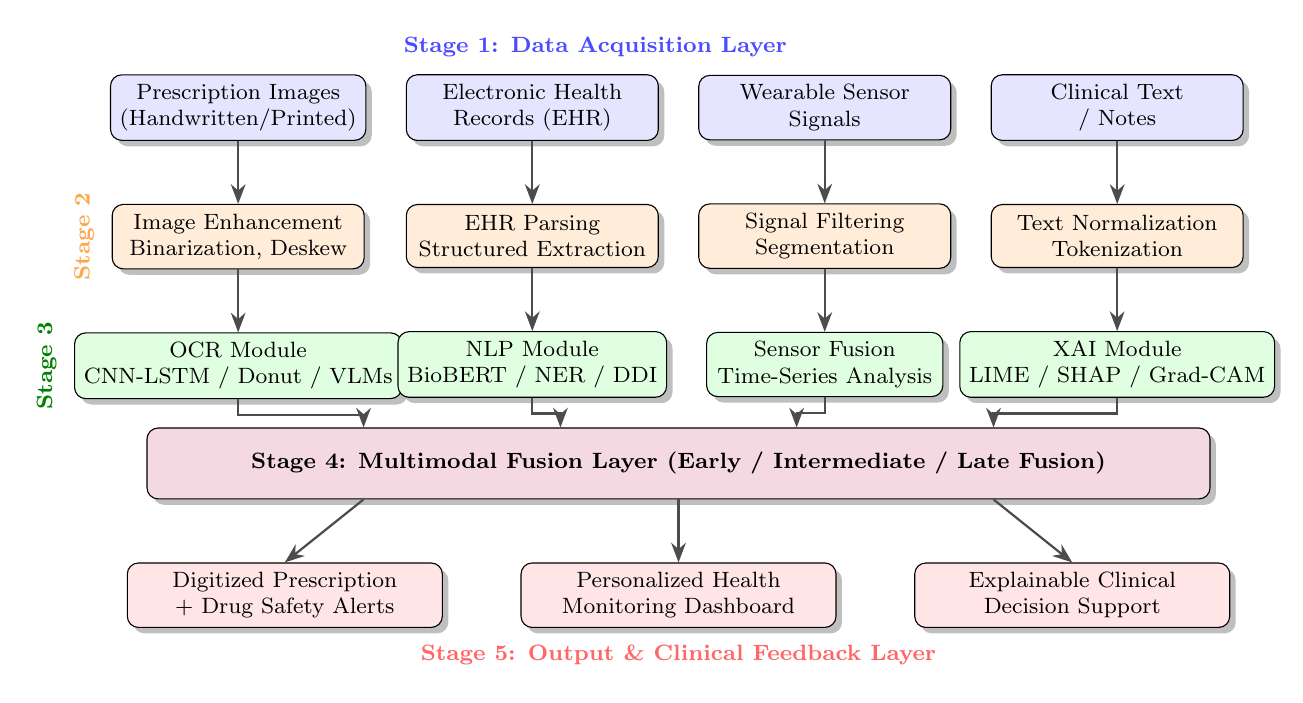
\begin{tikzpicture}[
    node distance=0.6cm and 0.8cm,
    inputbox/.style={draw, rounded corners, fill=blue!10, minimum width=3.2cm, minimum height=0.8cm, align=center, font=\footnotesize, drop shadow},
    processbox/.style={draw, rounded corners, fill=orange!15, minimum width=3.2cm, minimum height=0.8cm, align=center, font=\footnotesize, drop shadow},
    aibox/.style={draw, rounded corners, fill=green!12, minimum width=3.0cm, minimum height=0.8cm, align=center, font=\footnotesize, drop shadow},
    fusionbox/.style={draw, rounded corners, fill=purple!15, minimum width=13.5cm, minimum height=0.9cm, align=center, font=\footnotesize\bfseries, drop shadow},
    outputbox/.style={draw, rounded corners, fill=red!10, minimum width=4.0cm, minimum height=0.8cm, align=center, font=\footnotesize, drop shadow},
    stagebox/.style={draw, dashed, rounded corners, fill=gray!5, inner sep=0.3cm},
    arrow/.style={-{Stealth[length=2.5mm]}, thick, color=black!70}
]

\node[inputbox] (rx) {Prescription Images\\(Handwritten/Printed)};
\node[inputbox, right=0.5cm of rx] (ehr) {Electronic Health\\Records (EHR)};
\node[inputbox, right=0.5cm of ehr] (wear) {Wearable Sensor\\Signals};
\node[inputbox, right=0.5cm of wear] (text) {Clinical Text\\/ Notes};

\node[above=0.1cm of ehr, xshift=0.8cm, font=\footnotesize\bfseries\color{blue!70}] {\textbf{Stage 1: Data Acquisition Layer}};


\node[processbox, below=0.8cm of rx] (p1) {Image Enhancement\\Binarization, Deskew};
\node[processbox, below=0.8cm of ehr] (p2) {EHR Parsing\\Structured Extraction};
\node[processbox, below=0.8cm of wear] (p3) {Signal Filtering\\Segmentation};
\node[processbox, below=0.8cm of text] (p4) {Text Normalization\\Tokenization};

\node[left=0.1cm of p1, font=\footnotesize\bfseries\color{orange!70}, rotate=90, anchor=south] {\textbf{Stage 2}};


\draw[arrow] (rx) -- (p1);
\draw[arrow] (ehr) -- (p2);
\draw[arrow] (wear) -- (p3);
\draw[arrow] (text) -- (p4);


\node[aibox, below=0.8cm of p1] (ocr) {OCR Module\\CNN-LSTM / Donut / VLMs};
\node[aibox, below=0.8cm of p2] (nlp) {NLP Module\\BioBERT / NER / DDI};
\node[aibox, below=0.8cm of p3] (sensor) {Sensor Fusion\\Time-Series Analysis};
\node[aibox, below=0.8cm of p4] (xai) {XAI Module\\LIME / SHAP / Grad-CAM};

\node[left=0.1cm of ocr, font=\footnotesize\bfseries\color{green!50!black}, rotate=90, anchor=south] {\textbf{Stage 3}};


\draw[arrow] (p1) -- (ocr);
\draw[arrow] (p2) -- (nlp);
\draw[arrow] (p3) -- (sensor);
\draw[arrow] (p4) -- (xai);


\node[fusionbox, below=0.8cm of $(nlp)!0.5!(sensor)$] (fusion) {Stage 4: Multimodal Fusion Layer (Early / Intermediate / Late Fusion)};


\draw[arrow] (ocr.south) -- ++(0,-0.2) -| ([xshift=-4cm]fusion.north);
\draw[arrow] (nlp.south) -- ++(0,-0.2) -| ([xshift=-1.5cm]fusion.north);
\draw[arrow] (sensor.south) -- ++(0,-0.2) -| ([xshift=1.5cm]fusion.north);
\draw[arrow] (xai.south) -- ++(0,-0.2) -| ([xshift=4cm]fusion.north);


\node[outputbox, below=0.8cm of fusion, xshift=-5cm] (out1) {Digitized Prescription\\+ Drug Safety Alerts};
\node[outputbox, below=0.8cm of fusion] (out2) {Personalized Health\\Monitoring Dashboard};
\node[outputbox, below=0.8cm of fusion, xshift=5cm] (out3) {Explainable Clinical\\Decision Support};


\draw[arrow] ([xshift=-4cm]fusion.south) -- (out1.north);
\draw[arrow] (fusion.south) -- (out2.north);
\draw[arrow] ([xshift=4cm]fusion.south) -- (out3.north);

\node[below=0.1cm of out2, font=\footnotesize\bfseries\color{red!60}] {\textbf{Stage 5: Output \& Clinical Feedback Layer}};

\end{tikzpicture}
\caption{Proposed MediXAI five-stage multimodal AI pipeline for prescription analysis and personalized health monitoring.}
\label{fig:pipeline}
\end{figure*}

\vspace{2em}

\begin{figure*}[!htbp]
\centering
\includegraphics[width=\textwidth]{workflow.png}
\caption{Workflow diagram illustrating the comprehensive data flow and processing stages within the MediXAI framework.}
\label{fig:workflow}
\end{figure*}

\vspace{2em}

\begin{figure*}[!htbp]
\centering
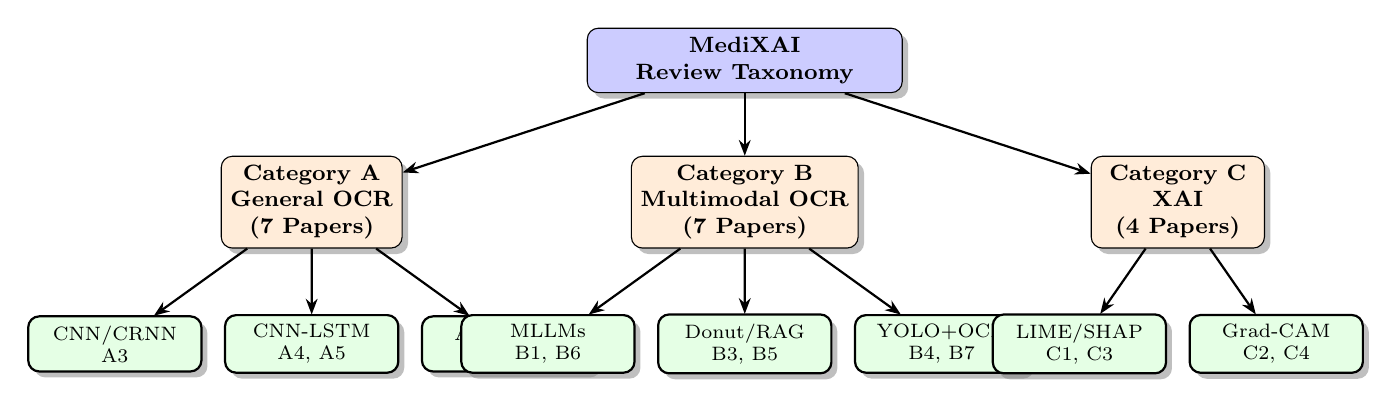
\begin{tikzpicture}[
    level 1/.style={sibling distance=5.5cm, level distance=1.8cm},
    level 2/.style={sibling distance=2.5cm, level distance=1.8cm},
    every node/.style={draw, rounded corners, align=center, font=\footnotesize, minimum width=2.2cm, minimum height=0.7cm, drop shadow},
    root/.style={fill=blue!20, font=\footnotesize\bfseries, minimum width=4cm},
    cat/.style={fill=orange!15, font=\footnotesize\bfseries},
    leaf/.style={fill=green!10, font=\scriptsize},
    edge from parent/.style={draw, -{Stealth[length=2mm]}, thick}
]

\node[root] {MediXAI\\Review Taxonomy}
    child { node[cat] {Category A\\General OCR\\(7 Papers)}
        child { node[leaf] {CNN/CRNN\\A3} }
        child { node[leaf] {CNN-LSTM\\A4, A5} }
        child { node[leaf] {ANN/MLP\\A7} }
    }
    child { node[cat] {Category B\\Multimodal OCR\\(7 Papers)}
        child { node[leaf] {MLLMs\\B1, B6} }
        child { node[leaf] {Donut/RAG\\B3, B5} }
        child { node[leaf] {YOLO+OCR\\B4, B7} }
    }
    child { node[cat] {Category C\\XAI\\(4 Papers)}
        child { node[leaf] {LIME/SHAP\\C1, C3} }
        child { node[leaf] {Grad-CAM\\C2, C4} }
    };

\end{tikzpicture}
\caption{Taxonomy of reviewed literature organized by thematic category and methodology.}
\label{fig:taxonomy}
\end{figure*}

\begin{figure}[!htbp]
\centering
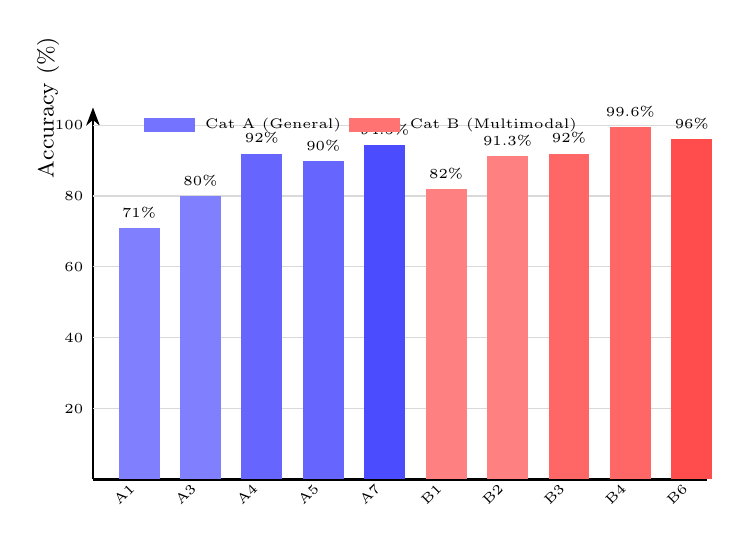
\begin{tikzpicture}[
    xscale=0.65, yscale=0.045
]

\draw[thick, -{Stealth}] (0,0) -- (0,105) node[left, font=\footnotesize, rotate=90, anchor=south, yshift=0.3cm] {Accuracy (\%)};
\draw[thick] (0,0) -- (12,0);


\foreach \y in {20,40,60,80,100} {
    \draw[gray!30, thin] (0,\y) -- (12,\y);
    \node[left, font=\tiny] at (0,\y) {\y};
}


\fill[blue!50] (0.5,0) rectangle (1.3,71);   \node[below, font=\tiny, rotate=45, anchor=east] at (0.9,0) {A1};
\fill[blue!50] (1.7,0) rectangle (2.5,80);   \node[below, font=\tiny, rotate=45, anchor=east] at (2.1,0) {A3};
\fill[blue!60] (2.9,0) rectangle (3.7,92);   \node[below, font=\tiny, rotate=45, anchor=east] at (3.3,0) {A4};
\fill[blue!60] (4.1,0) rectangle (4.9,90);   \node[below, font=\tiny, rotate=45, anchor=east] at (4.5,0) {A5};
\fill[blue!70] (5.3,0) rectangle (6.1,94.5); \node[below, font=\tiny, rotate=45, anchor=east] at (5.7,0) {A7};
\fill[red!50] (6.5,0) rectangle (7.3,82);    \node[below, font=\tiny, rotate=45, anchor=east] at (6.9,0) {B1};
\fill[red!50] (7.7,0) rectangle (8.5,91.3);  \node[below, font=\tiny, rotate=45, anchor=east] at (8.1,0) {B2};
\fill[red!60] (8.9,0) rectangle (9.7,92);    \node[below, font=\tiny, rotate=45, anchor=east] at (9.3,0) {B3};
\fill[red!60] (10.1,0) rectangle (10.9,99.6);\node[below, font=\tiny, rotate=45, anchor=east] at (10.5,0) {B4};
\fill[red!70] (11.3,0) rectangle (12.1,96);  \node[below, font=\tiny, rotate=45, anchor=east] at (11.7,0) {B6};


\node[above, font=\tiny] at (0.9,71) {71\%};
\node[above, font=\tiny] at (2.1,80) {80\%};
\node[above, font=\tiny] at (3.3,92) {92\%};
\node[above, font=\tiny] at (4.5,90) {90\%};
\node[above, font=\tiny] at (5.7,94.5) {94.5\%};
\node[above, font=\tiny] at (6.9,82) {82\%};
\node[above, font=\tiny] at (8.1,91.3) {91.3\%};
\node[above, font=\tiny] at (9.3,92) {92\%};
\node[above, font=\tiny] at (10.5,99.6) {99.6\%};
\node[above, font=\tiny] at (11.7,96) {96\%};


\fill[blue!55] (1,98) rectangle (2,102); \node[right, font=\tiny] at (2,100) {Cat A (General)};
\fill[red!55] (5,98) rectangle (6,102); \node[right, font=\tiny] at (6,100) {Cat B (Multimodal)};

\end{tikzpicture}
\caption{Accuracy comparison across reviewed prescription OCR studies.}
\label{fig:accuracy}
\end{figure}

\subsection{Design Rationale}

The five-stage architecture of MediXAI is motivated by the following observations from the reviewed literature:

\begin{itemize}
    \item \textbf{OCR is necessary but insufficient}: All Category A and B papers demonstrate that prescription OCR alone cannot ensure medication safety. Post-OCR NLP validation, drug interaction checking, and semantic verification are essential additional layers.

    \item \textbf{Multimodal fusion improves clinical relevance}: The comparison between Category A (unimodal) and Category B (multimodal) papers shows that incorporating multiple data sources and model architectures generally yields higher accuracy and more robust performance.

    \item \textbf{Explainability is a clinical requirement}: Category C papers consistently emphasize that AI systems without transparent reasoning mechanisms face significant barriers to clinical adoption.

    \item \textbf{Monitoring completes the clinical loop}: Prescription analysis produces a treatment plan, but monitoring determines whether that plan is effective and safe. This feedback loop is essential for personalized medicine.
\end{itemize}












\section{Challenges and Research Gaps}
\label{sec:challenges}

The following critical challenges and research gaps have been identified. Figure \ref{fig:researchgap} illustrates the core divergence between current isolated systems and the required integrated MediXAI approach.

\vspace{1em}

\begin{figure*}[!htbp]
\centering
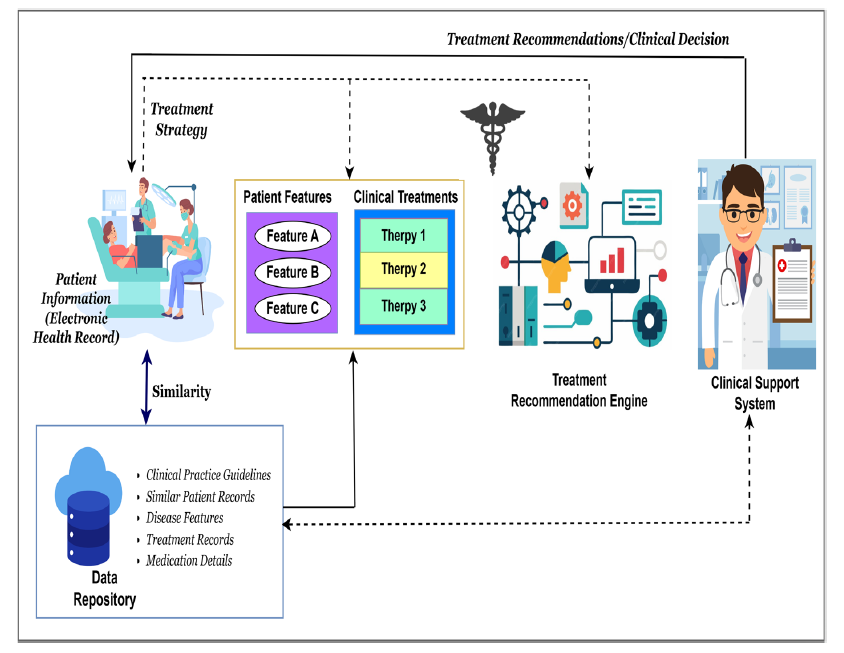
\includegraphics[width=\textwidth]{researchgap.png}
\caption{Visual representation of the research gap: bridging the divide between isolated current systems and the unified MediXAI framework.}
\label{fig:researchgap}
\end{figure*}

\subsection{Handwriting Variability and Image Quality}

The most frequently cited error source across 16 of 18 papers is poor image quality including faded, blurred, and noisy scans. Physician handwriting variability remains the fundamental challenge for prescription OCR. Even the most advanced VLM-based systems achieve only 82--96\% accuracy, which is insufficient for unsupervised clinical deployment where a single character error can change a medication name entirely \cite{mankash2024mirage,intuitionlabs2026pharma,gifu2022aibacked}.

\subsection{Absence of Cross-Modal Fusion}

No reviewed paper combines prescription OCR with wearable health monitoring data in a unified framework. Current systems operate in isolation: OCR systems process prescriptions, monitoring systems track vital signs, and NLP systems analyze clinical text. The MediXAI framework addresses this gap by proposing an integrated pipeline, but significant engineering and research challenges remain in implementing effective cross-modal fusion for these heterogeneous data types.

\subsection{Insufficient Clinical Validation}

Only 3 of 18 papers report any form of real-world clinical deployment or validation. The majority of studies evaluate on benchmark or proprietary datasets without testing in actual hospital workflows \cite{intuitionlabs2026pharma}. This gap between laboratory performance and clinical utility is a major barrier to adoption.

\subsection{Limited Multilingual Support}

Most reviewed systems are English-only. Only two papers address multilingual prescriptions: the YOLO-based system for Bangla prescriptions \cite{chandra2019prescription} and MIRAGE for Indian prescriptions \cite{mankash2024mirage}. Given that illegible prescriptions are most prevalent in developing countries with diverse linguistic environments, multilingual OCR is a critical unmet need.

\subsection{Data Privacy and Security}

Healthcare data is highly sensitive and subject to stringent regulations including HIPAA and GDPR. Only one reviewed paper \cite{babu2024aidriven} explicitly proposes Federated Learning for privacy-preserving medical AI. The remaining studies either use public benchmark datasets or do not address privacy considerations, leaving a significant gap in responsible AI deployment.

\subsection{Lack of Integrated XAI}

No reviewed paper integrates explainable AI techniques with prescription OCR pipelines. Category C papers demonstrate XAI effectiveness for medical imaging and disease detection, but these techniques have not been applied to explain prescription recognition decisions, drug interaction alerts, or personalized monitoring recommendations. This represents a key opportunity for MediXAI.

\subsection{Computational Cost and Scalability}

Advanced MLLM-based approaches such as MIRAGE require substantial computational resources (13 days training on 6$\times$A6000 GPUs) \cite{mankash2024mirage}. The pharma benchmark study \cite{intuitionlabs2026pharma} also noted high computational costs and slower inference speeds for VLMs. Deploying these models in resource-constrained healthcare settings remains challenging.

\begin{table}[!htbp]
\centering
\caption{Summary of Identified Research Gaps}
\label{tab:gaps}
\footnotesize
\begin{tabular}{|c|p{3.5cm}|p{3.2cm}|}
\hline
\textbf{No.} & \textbf{Research Gap} & \textbf{Papers Affected} \\
\hline
1 & No cross-modal prescription-to-monitoring fusion & All 18 papers \\
\hline
2 & Insufficient real-world clinical validation & 15 of 18 papers \\
\hline
3 & Limited multilingual support & 14 of 18 papers \\
\hline
4 & No XAI integration with prescription OCR & All Cat A \& B papers \\
\hline
5 & Data privacy not addressed & 17 of 18 papers \\
\hline
6 & High computational cost for MLLMs & B1, B3, B5, B6 \\
\hline
7 & No drug interaction detection in OCR pipeline & 16 of 18 papers \\
\hline
8 & Accuracy insufficient for unsupervised clinical use & All Cat A \& B papers \\
\hline
\end{tabular}
\end{table}

\section{Future Research Directions}
\label{sec:future}

Based on the identified research gaps, the following future research directions are recommended for advancing the MediXAI framework:

\subsection{Unified Multimodal Architecture}

Future systems should develop end-to-end multimodal architectures that can simultaneously process prescription images, EHR data, wearable sensor streams, and clinical text within a single model. Multimodal transformers with cross-attention mechanisms and shared tokenization strategies represent promising approaches for achieving this unification. By sharing latent representations across modalities, the model can learn cross-modal dependencies that are currently missed by isolated systems. This architectural shift requires significant advancements in model capacity and training efficiency but promises to deliver a truly holistic view of patient health.

\subsection{Advanced Vision Encoders for Medical Handwriting}

The MIRAGE study \cite{mankash2024mirage} identified the vision encoder as the primary bottleneck in MLLM-based prescription OCR. Future work should explore specialized vision encoders trained on medical handwriting, including models such as TrOCR, SigLIP with medical fine-tuning, and hybrid architectures combining handwriting-specific feature extractors with general-purpose language models. Creating a specialized corpus of medical handwriting with fine-grained annotations for stroke order and ligatures could significantly improve encoder performance on complex cursive text.

\subsection{Integrated Drug Safety Layer}

Future MediXAI implementations should incorporate real-time drug-drug interaction detection immediately after prescription digitization. This requires integrating biomedical NLP models such as BioBERT with comprehensive drug interaction databases to automatically flag potentially dangerous medication combinations before dispensing. Furthermore, integrating patient-specific genomic data could enable pharmacogenomic safety checks, predicting adverse reactions based on individual metabolic profiles rather than just population averages.

\subsection{Federated Learning for Privacy-Preserving Healthcare AI}

To address data privacy concerns while leveraging distributed hospital data, future research should implement federated learning frameworks that enable model training across multiple institutions without centralizing raw patient data. Differential privacy and secure multi-party computation can provide additional privacy guarantees. Developing efficient federated learning protocols for large multimodal models like VLMs remains a significant technical challenge that requires novel algorithmic approaches to communication efficiency and aggregation strategies.

\subsection{Clinical Validation and Prospective Studies}

The field urgently needs prospective clinical validation studies that evaluate MediXAI-type systems in actual hospital pharmacies and clinical workflows. These studies should measure not only technical accuracy but also clinical impact metrics including medication error reduction rates, pharmacist workload reduction, and patient safety outcomes. Long-term observational studies are necessary to assess the sustained impact of these systems on treatment adherence and health outcomes, moving beyond the snapshot evaluations typical of current academic research.

\subsection{Explainable Prescription AI}

Future research should develop XAI techniques specifically designed for prescription analysis, such as attention visualization over prescription regions, confidence scoring for individual extracted entities, and uncertainty estimation that triggers human review for ambiguous cases. The integration of LIME and SHAP with OCR output layers can provide character-level and word-level explanation of recognition decisions. Moreover, counterfactual explanations could help clinicians understand and trust the AI's reasoning process in critical safety scenarios.

\subsection{Multilingual and Low-Resource Language Support}

Expanding prescription OCR to support multilingual and low-resource languages including Bangla, Hindi, Urdu, Arabic, and various African languages is essential for global healthcare impact. Transfer learning from high-resource languages and data augmentation using synthetic handwriting generation are promising strategies. Collaborative efforts to build open, multilingual medical handwriting datasets will be crucial to democratize access to these AI tools and ensure that benefits are not restricted to English-speaking regions.

\subsection{Edge Deployment and Mobile Integration}

For real-world adoption in resource-constrained settings, MediXAI models must be optimized for edge deployment on mobile devices and embedded systems. Model distillation, quantization, and pruning techniques can reduce computational requirements while maintaining acceptable accuracy levels. Developing lightweight versions of large multimodal models that can run on standard smartphones or point-of-care devices will enable real-time prescription checking in remote clinics and home care settings, significantly extending the reach of these safety systems.

\section{Conclusion}
\label{sec:conclusion}

This review paper has presented a comprehensive analysis of the MediXAI concept---a multimodal AI framework for prescription analysis and personalized health monitoring. Through the systematic examination of eighteen research papers published between 2020 and 2026 across three thematic categories, the review has provided a detailed understanding of the current state of the art, persistent challenges, and critical research gaps in this domain.

The comparative analysis revealed several key findings. In the domain of handwritten prescription OCR, general approaches using CNN, LSTM, and hybrid architectures achieve moderate accuracy ranging from 71\% to 94.5\%, while advanced multimodal approaches employing Vision-Language Models and transformer-based architectures push accuracy to 82--99.6\%. However, even the highest-performing systems remain insufficient for fully unsupervised clinical deployment due to the safety-critical nature of medication prescriptions. The explainable AI literature demonstrates that LIME, SHAP, and Grad-CAM are effective frameworks for enhancing model transparency, but these techniques have not yet been integrated with prescription OCR pipelines.

The most significant research gap identified is the absence of cross-modal fusion architectures that connect prescription digitization with continuous patient health monitoring. Current systems operate in isolation, processing individual data modalities without leveraging the complementary information available from other sources. The proposed MediXAI five-stage pipeline addresses this gap by providing a conceptual architecture that integrates data acquisition, preprocessing, AI processing, multimodal fusion, and explainable clinical feedback into a unified framework.

The overall evidence suggests that a well-designed MediXAI system has the potential to significantly reduce prescription ambiguity, support more adaptive chronic disease monitoring, and improve healthcare decision-making. The most promising future implementations will be those that successfully integrate multimodal data processing, generate explainable and trustworthy outputs, ensure patient data privacy through federated learning, and undergo rigorous prospective clinical validation. This review provides a structured foundation and actionable roadmap for researchers and practitioners working toward the realization of such systems.


\bibliographystyle{IEEEtran}
\bibliography{references}

\end{document} 